\documentclass[a4paper]{report}
% Some basic packages
\usepackage[utf8]{inputenc}
\usepackage[T1]{fontenc}
\usepackage{textcomp}
\usepackage[english]{babel}
\usepackage{url}
\usepackage{graphicx}
\usepackage{float}
\usepackage{booktabs}
\usepackage{enumitem}

\pdfminorversion=7

% Don't indent paragraphs, leave some space between them
\usepackage{parskip}

% Hide page number when page is empty
\usepackage{emptypage}
\usepackage{subcaption}
\usepackage{multicol}
\usepackage{xcolor}

% Other font I sometimes use.
% \usepackage{cmbright}

% Math stuff
\usepackage{amsmath, amsfonts, mathtools, amsthm, amssymb}
% Fancy script capitals
\usepackage{mathrsfs}
\usepackage{cancel}
% Bold math
\usepackage{bm}
% Some shortcuts
\newcommand\N{\ensuremath{\mathbb{N}}}
\newcommand\R{\ensuremath{\mathbb{R}}}
\newcommand\Z{\ensuremath{\mathbb{Z}}}
\renewcommand\O{\ensuremath{\emptyset}}
\newcommand\Q{\ensuremath{\mathbb{Q}}}
\newcommand\C{\ensuremath{\mathbb{C}}}
\renewcommand\L{\ensuremath{\mathcal{L}}}

% Package for Petri Net drawing
\usepackage[version=0.96]{pgf}
\usepackage{tikz}
\usetikzlibrary{arrows,shapes,automata,petri}
\usepackage{tikzit}
\input{petri_nets_style.tikzstyles}

% Easily typeset systems of equations (French package)
\usepackage{systeme}

% Put x \to \infty below \lim
\let\svlim\lim\def\lim{\svlim\limits}

%Make implies and impliedby shorter
\let\implies\Rightarrow
\let\impliedby\Leftarrow
\let\iff\Leftrightarrow
\let\epsilon\varepsilon

% Add \contra symbol to denote contradiction
\usepackage{stmaryrd} % for \lightning
\newcommand\contra{\scalebox{1.5}{$\lightning$}}

% \let\phi\varphi

% Command for short corrections
% Usage: 1+1=\correct{3}{2}

\definecolor{correct}{HTML}{009900}
\newcommand\correct[2]{\ensuremath{\:}{\color{red}{#1}}\ensuremath{\to }{\color{correct}{#2}}\ensuremath{\:}}
\newcommand\green[1]{{\color{correct}{#1}}}

% horizontal rule
\newcommand\hr{
    \noindent\rule[0.5ex]{\linewidth}{0.5pt}
}

% hide parts
\newcommand\hide[1]{}

% si unitx
\usepackage{siunitx}
\sisetup{locale = FR}

% Environments
\makeatother
% For box around Definition, Theorem, \ldots
\usepackage{mdframed}
\mdfsetup{skipabove=1em,skipbelow=0em}
\theoremstyle{definition}
\newmdtheoremenv[nobreak=true]{definitie}{Definitie}
\newmdtheoremenv[nobreak=true]{eigenschap}{Eigenschap}
\newmdtheoremenv[nobreak=true]{gevolg}{Gevolg}
\newmdtheoremenv[nobreak=true]{lemma}{Lemma}
\newmdtheoremenv[nobreak=true]{propositie}{Propositie}
\newmdtheoremenv[nobreak=true]{stelling}{Stelling}
\newmdtheoremenv[nobreak=true]{wet}{Wet}
\newmdtheoremenv[nobreak=true]{postulaat}{Postulaat}
\newmdtheoremenv{conclusie}{Conclusie}
\newmdtheoremenv{toemaatje}{Toemaatje}
\newmdtheoremenv{vermoeden}{Vermoeden}
\newtheorem*{herhaling}{Herhaling}
\newtheorem*{intermezzo}{Intermezzo}
\newtheorem*{notatie}{Notatie}
\newtheorem*{observatie}{Observatie}
\newtheorem*{exe}{Exercise}
\newtheorem*{opmerking}{Opmerking}
\newtheorem*{praktisch}{Praktisch}
\newtheorem*{probleem}{Probleem}
\newtheorem*{terminologie}{Terminologie}
\newtheorem*{toepassing}{Toepassing}
\newtheorem*{uovt}{UOVT}
\newtheorem*{vb}{Voorbeeld}
\newtheorem*{vraag}{Vraag}

\newmdtheoremenv[nobreak=true]{definition}{Definition}
\newtheorem*{eg}{Example}
\newtheorem*{notation}{Notation}
\newtheorem*{previouslyseen}{As previously seen}
\newtheorem*{remark}{Remark}
\newtheorem*{note}{Note}
\newtheorem*{problem}{Problem}
\newtheorem*{observe}{Observe}
\newtheorem*{property}{Property}
\newtheorem*{intuition}{Intuition}
\newmdtheoremenv[nobreak=true]{prop}{Proposition}
\newmdtheoremenv[nobreak=true]{theorem}{Theorem}
\newmdtheoremenv[nobreak=true]{corollary}{Corollary}

% End example and intermezzo environments with a small diamond (just like proof
% environments end with a small square)
\usepackage{etoolbox}
\AtEndEnvironment{vb}{\null\hfill$\diamond$}%
\AtEndEnvironment{intermezzo}{\null\hfill$\diamond$}%
% \AtEndEnvironment{opmerking}{\null\hfill$\diamond$}%

% Fix some spacing
% http://tex.stackexchange.com/questions/22119/how-can-i-change-the-spacing-before-theorems-with-amsthm
\makeatletter
\def\thm@space@setup{%
  \thm@preskip=\parskip \thm@postskip=0pt
}


% Exercise 
% Usage:
% \exercise{5}
% \subexercise{1}
% \subexercise{2}
% \subexercise{3}
% gives
% Exercise 5
%   Exercise 5.1
%   Exercise 5.2
%   Exercise 5.3
\newcommand{\exercise}[1]{%
    \def\@exercise{#1}%
    \subsection*{Exercise #1}
}

\newcommand{\subexercise}[1]{%
    \subsubsection*{Exercise \@exercise.#1}
}


% \lecture starts a new lecture (les in dutch)
%
% Usage:
% \lecture{1}{di 12 feb 2019 16:00}{Inleiding}
%
% This adds a section heading with the number / title of the lecture and a
% margin paragraph with the date.

% I use \dateparts here to hide the year (2019). This way, I can easily parse
% the date of each lecture unambiguously while still having a human-friendly
% short format printed to the pdf.

\usepackage{xifthen}
\def\testdateparts#1{\dateparts#1\relax}
\def\dateparts#1 #2 #3 #4 #5\relax{
    \marginpar{\small\textsf{\mbox{#1 #2 #3 #5}}}
}

\def\@lecture{}%
\newcommand{\lecture}[3]{
    \ifthenelse{\isempty{#3}}{%
        \def\@lecture{Lecture #1}%
    }{%
        \def\@lecture{Lecture #1: #3}%
    }%
    \subsection*{\@lecture}
    \marginpar{\small\textsf{\mbox{#2}}}
}



% These are the fancy headers
\usepackage{fancyhdr}
\pagestyle{fancy}

% LE: left even
% RO: right odd
% CE, CO: center even, center odd
% My name for when I print my lecture notes to use for an open book exam.
% \fancyhead[LE,RO]{Gilles Castel}

\fancyhead[RO,LE]{\@lecture} % Right odd,  Left even
\fancyhead[RE,LO]{}          % Right even, Left odd

\fancyfoot[RO,LE]{\thepage}  % Right odd,  Left even
\fancyfoot[RE,LO]{}          % Right even, Left odd
\fancyfoot[C]{\leftmark}     % Center

\makeatother




% Todonotes and inline notes in fancy boxes
\usepackage{todonotes}
\usepackage{tcolorbox}

% Make boxes breakable
\tcbuselibrary{breakable}

% Verbetering is correction in Dutch
% Usage: 
% \begin{verbetering}
%     Lorem ipsum dolor sit amet, consetetur sadipscing elitr, sed diam nonumy eirmod
%     tempor invidunt ut labore et dolore magna aliquyam erat, sed diam voluptua. At
%     vero eos et accusam et justo duo dolores et ea rebum. Stet clita kasd gubergren,
%     no sea takimata sanctus est Lorem ipsum dolor sit amet.
% \end{verbetering}
\newenvironment{verbetering}{\begin{tcolorbox}[
    arc=0mm,
    colback=white,
    colframe=green!60!black,
    title=Opmerking,
    fonttitle=\sffamily,
    breakable
]}{\end{tcolorbox}}

% Noot is note in Dutch. Same as 'verbetering' but color of box is different
\newenvironment{noot}[1]{\begin{tcolorbox}[
    arc=0mm,
    colback=white,
    colframe=white!60!black,
    title=#1,
    fonttitle=\sffamily,
    breakable
]}{\end{tcolorbox}}




% Figure support as explained in my blog post.
\usepackage{import}
\usepackage{xifthen}
\usepackage{pdfpages}
\usepackage{transparent}
\newcommand{\incfig}[1]{%
    \def\svgwidth{\columnwidth}
    \import{./figures/}{#1.pdf_tex}
}

% Fix some stuff
% %http://tex.stackexchange.com/questions/76273/multiple-pdfs-with-page-group-included-in-a-single-page-warning
\pdfsuppresswarningpagegroup=1


% My name
\author{Bruno M. Pacheco}

 
\begin{document}
 
\title{Lista 1}
\author{Bruno M. Pacheco\\
DAS 5142 - Sistemas Dinâmicos}
 
\maketitle
 
\exercise{1}

Podemos analisar o comportamento dos sistemas através de seus pontos de equilíbrio.

\subexercise{i}

\begin{align*}
    \dot{x} = 0 \implies y = x\left( x^2 + y^2 -1 \right) \\
    \implies \dot{y} = 0 = x\left( x^2 + y^2 -1 \right)^2 + x
.\end{align*}
Como $\left( x^2 + y^2 -1 \right)^2 \ge 0$, o único ponto de equilíbrio é $(\overline{x}, \overline{y}) = (0,0)$. Assim, o único diagrama possível é o \textbf{diagrama B}.

\subexercise{ii}

De forma mais evidente, para este sistema os pontos de equilíbrio são $y=0$ e $x \in {-1,1}$, portanto o \textbf{diagrama C} é o único possível.

\subexercise{iii}

Aqui, a condição do ponto de equilíbrio para a segunda equação implica que $x=0$ \emph{ou} $y = \pm 1$. Para o primeiro caso, temos que, claramente, $\dot{y}=0 \implies y=0$, assim temos um ponto de equilíbrio em $\left( 0,0 \right) $. No segundo caso, temos, se $y=1$,
\begin{align*}
    &\dot{x}=0=\left( 1 + \frac{x}{5} \right) \left( 1-x^2 \right) \\
    &\implies 1 -x^2 + \frac{x}{5} - \frac{x^3}{5} = 0 \\
,\end{align*}
que possui soluções em $x=\pm 1$. Já se $y=-1$, temos de forma semelhante  \[
-1 + x^2+ \frac{x}{5} - \frac{x^3}{5} = 0
,\] que também possui soluções em $x=\pm 1$. Portanto, o único diagrama possível é o  \textbf{diagrama C}.

\subexercise{iv}

Além de $\left( x,y \right) = \left( 0,0 \right) $, também temos outros pontos de equilíbrio quando somente um dos estados é nulo. Quando $x=0$ mas $y\neq 0$, temos ponto de equilíbrio se \[
    0.6\left( 1-y+0.3x \right) y = 0
,\] ou seja, em $y=1$.

Se $y=0$ mas $x\neq 0$, então temos \[
0.4\left( 1-x+2y \right) x = 0 \implies x=1
.\]

Já se ambos são não-nulos, podemos encontrar um ponto de equilíbrio se \[
1-x+2y = 0 = 1-y+0.3x
,\] o que nos leva a manipulação
\begin{align*}
    &\left( 1-x+2y \right) + 2\left( 1-y+0.3x \right) = 0 \\
    &\implies 3-x+0.6x = 0 \\
    &\implies x = 7,5 \\
    &1-x+2y = 0 \\
    &\implies 1-7,5 + 2y = 0 \\
    &\implies y=3,25 \\
,\end{align*}
ou seja, como esperado, o diagrama referente é o \textbf{diagrama A}.

\exercise{2}

\subexercise{a}

Obviamente, temos um ponto de equilíbrio em $x=y=0$. Nesse ponto de equilíbrio, temos  \[
    J = \begin{bmatrix} 3 & 0 \\ 0 & 2 \end{bmatrix} 
,\] que possui autovalores positivos, portanto, podemos afirmar que o ponto de equilíbrio é instável, o que condiz com a nossa intuição sobre o sistema.

Além disso, para o caso $x=0$ e $y\neq 0$, temos \[
\dot{y} = 0 \implies 0 = 2y - y^2 \implies y = 2
,\] um ponto de equilíbrio com jacobiana \[
J = \begin{bmatrix} 
    -1 & 0 \\
    -2 & -2
\end{bmatrix} 
,\] ou seja, um ponto de equilíbrio também estável, uma vez que os autovalores de J são negativos ($-1$ e  $-2$).

Já para $y=0$ e $x\neq 0$, temos de forma similar um ponto de equilíbrio se $x=3$, com Jacobiana  \[
J = \begin{bmatrix} 
    -3 & -6 \\
    0 & -1
\end{bmatrix} 
,\] que também nos garante estabilidade por ter autovalores negativos.

\subexercise{b}

\begin{figure}[H]
    \centering
    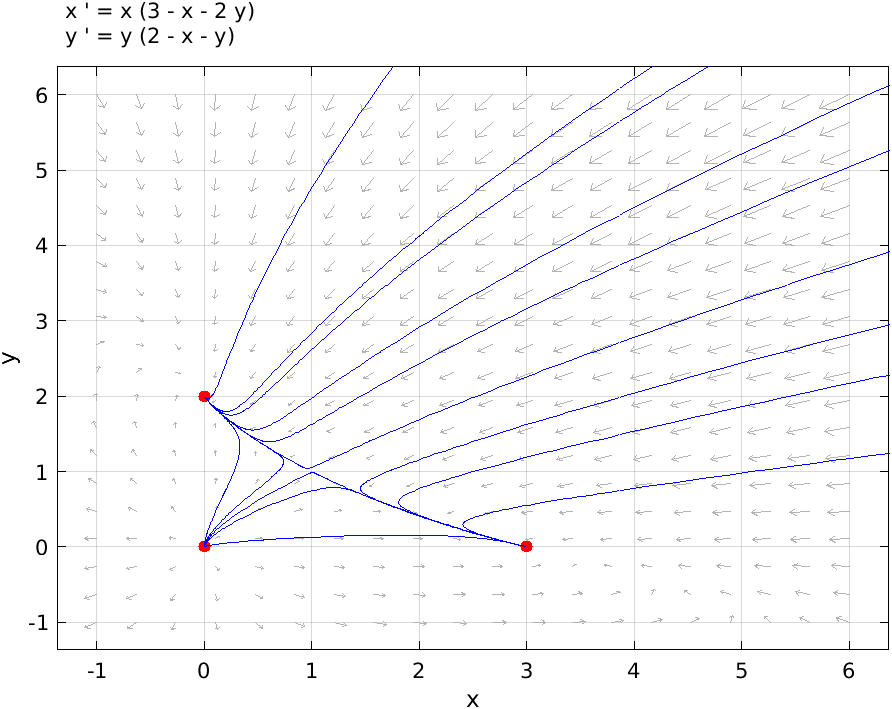
\includegraphics[width=0.6\textwidth]{lista1_2b.png}
    \caption{Pontos de equilíbrio e regiões de atração.}
    \label{fig:lista1_2b-png}
\end{figure}

\subexercise{c}

Vemos que se existe qualquer população das duas espécies, a tendência é a de que somente uma delas sobreviva e sua população estabilize, indicada pelos pontos de equilíbrio estáveis.

\exercise{3}

\subexercise{a}

Para esse modelo, o único ponto de equilíbrio em função dos parâmetros $a$ e $b$ é
\begin{align*}
    \dot{x} = \dot{y} = 0 \\
    &\implies\left( -x + ay +x^2y \right) + \left( b-ay-x^2y \right) =0 \\
    &\implies x = b \\
    &\implies 0=b-ay-b^2y \\
    &\implies y = \frac{b}{a+b^2}
.\end{align*}

Agora, podemos ver que a Jacobiana desse sistema é \[
J = \begin{bmatrix} 
    -1 +2xy & a+x^2 \\
    -2xy & -a -x^2
\end{bmatrix} 
,\] que no ponto de equilíbrio é \[
\begin{bmatrix} 
    -1 +\frac{2b^2}{b^2+ a} & a+b^2 \\
    -\frac{2b^2}{b^2 + a} & -(a +b^2)
\end{bmatrix} 
.\] Assim, através do traço e do determinante dessa matriz podemos encontrar o polinômio característico $P\left( \lambda \right)$ do sistema
\begin{align*}
    det(J) &= -1 \left( -1 + \frac{2b^2}{b^2+a} \right) \left(a+b^2  \right) + \left(    \frac{2b^2}{b^2+a}\right) \left( a+b^2 \right) = a+b^2 > 0\\
    T(J) &= -1 + \frac{2b^2}{b^2+a} -\left( a+b^2 \right) = \frac{a + a^2 - b^2 +2ab^2 + b^{4}}{a+b^2}\\
	 &\implies P\left( \lambda \right) = \lambda^2 + \left( a + a^2 - b^2 +2ab^2 + b^{4} \right) \lambda + \left( a+b^2 \right)
.\end{align*}

Assim, podemos concluir que a estabilidade do ponto de equilíbrio depende do valor do coeficiente associado ao termo de primeiro grau do polinômio característico, sendo estável se esse é positivo, e instável mas com um ciclo limite estável se for negativo.

\subexercise{b}

À esquerda do traço temos a zona em que o ponto de equilíbrio é instável, enquanto à direita temos a zona de estabilidade. Assim, temos sobre o ponto nulo do traço uma bifurcação de Hopf.

\exercise{4}

\subexercise{a}

Temos \[
\frac{\partial N}{\partial t} = 0 = rN\left( \frac{N}{k_0}-1 \right) \left( 1-\frac{N}{k} \right) 
,\] ou seja, os pontos de equilíbrio são $\overline{N} \in \left\{ 0, k=0, k \right\}$, conforme o esperado. Agora, se $\frac{\partial N}{\partial t} = f(N)$, \[
f'(N) = r\left( \frac{N}{k_0}-1 \right) \left( 1-\frac{N}{k} \right) +rN\left( \frac{1}{k_0} \right) \left( 1-\frac{N}{k} \right) + rN\left( \frac{N}{k_0}-1 \right) \left( -\frac{1}{k} \right) -q
,\] e, portanto, \[
f'(\overline{N}) = \begin{cases}
    -r-q, & N=0 \\
    r\left( 1-\frac{k_0}{k} \right) -q & N=k_0 \\
    r\left( 1-\frac{k}{k_0} \right) -q & N=k
\end{cases}
.\] Considerando que $r>0$ e $q=0$, o ponto de equilíbrio em $N=0$ é claramente estável, enquanto em $N=k_0$ temos um ponto de equilíbrio instável, pois $1-\frac{k_0}{k}>0$ uma vez que $k_0<k$, enquanto em $N=k$ será estável pelo mesmo motivo.

\subexercise{b}

Considerando a ação da pesca no sistema, temos
\begin{align*}
    rN\left( \frac{N}{k_0}-1 \right) \left( 1-\frac{N}{k} \right) -qN = 0 \\
    \implies N^2 - \left( k+k_0 \right) N +k_0k +\frac{q}{r}k_0k = 0
,\end{align*}
assim podemos observar que o efeito do quociente $\frac{q}{r}$ é o de aproximar os pontos de equilíbrio não nulos.

Note que o resultado acima não considera o ponto de equilíbrio trivial $N=0$, que se mantém.

\subexercise{c}

Para analisar o efeito do parâmetro $q$, analisou-se seu impacto na relação entre a quantidade de peixes e a taxa de variação. Pode-se visualizar essa relação na figura abaixo.

\begin{figure}[H]
    \centering
    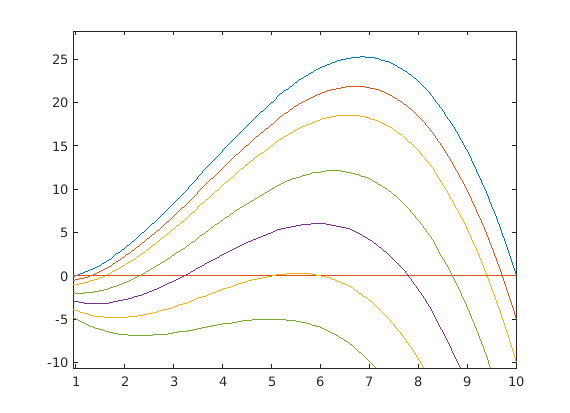
\includegraphics[width=0.6\textwidth]{lista1_4c.png}
    \caption{Relação entre $\frac{\partial N}{\partial t} $ e $N$ em função do parâmetro $q$.}
    \label{fig:lista1_4b-png}
\end{figure}

Vê-se que, conforme aumentamos o parâmetro $q$, a curva que representa a taxa de variação da população pelo seu número diminui. Ou seja, podemos encontrar os pontos de equilíbrio graficamente pelo cruzamento entre essas curvas e a reta em $\frac{\partial N}{\partial t} =0$. Ainda mais, sabemos que se a curva é crescente nesse ponto o ponto de equilíbrio é instável, sendo estável do contrário. Assim, podemos ver que quando $q>4.05$, não existe mais ponto de equilíbrio estável no sistema, fora $N=0$.

\subexercise{d}

Sabendo que o ponto de equilíbrio crítico é em $\frac{k_0+k}{2}$, determinou-se o valor crítico para $q$ através da equação (1). O esboço dos pontos de equilíbrio pode ser visto abaixo.

\begin{figure}[H]
    \centering
    \includegraphics[width=0.6\textwidth]{lista1_4d.pdf}
    \caption{Esboço dos pontos de equilíbrio do sistema.}
    \label{fig:lista1_4d-pdf}
\end{figure}

Vemos que quando existe uma pesca predatória excessiva, o sistema tende à zerar a sua população de peixes, portante deve-se manter a pesca em valores inferiores a $q=4.05$ para que exista uma população de peixes que consiga se reproduzir.

\exercise{5}

\subexercise{a}

Para $\mu=0$ temos o sistema representado pela equação \[
\frac{\partial T}{\partial t} = T^3 - T
,\] que possui equilíbrios em $T \in \left\{ -1, 0, 1 \right\} $. Agora, veja que \[
\frac{\partial f}{\partial T} = 3T^2 -1
,\] o que nos permite concluir que somente o equilíbrio em $T=0$ é estável.

\subexercise{b}

Para valores iniciais de temperatura fora do intervalo $[-1,1]$, o sistema diverge. Pode-se concluir isso a partir da curva apresentada, que nos indica que $\frac{\partial T}{\partial t} > 0 \forall T>1 \implies T \to \infty$ e também $\frac{\partial T}{\partial t} < 0 \forall T < -1 \implies T \to -\infty$.

\subexercise{c}

Analisando o problema de forma gráfica, sabemos que a influência do parâmetro $\mu$ é a de deslocar a curva apresentada no enunciado ao longo do eixo $f(T)$. Como também sabemos que as raízes da equação são a interseção da curva e o eixo das abscissas, podemos concluir que, para variações positivas do parâmetro $\mu$, as raízes nula e positiva se atraem enquanto a raiz negativa diverge, até que as duas raízes positivas se encontrem e, após, tornem-se uma raiz imaginária. Esse comportamento pode ser observado no esboço da figura abaixo.

\begin{figure}[H]
    \centering
    \includegraphics[width=0.6\textwidth]{lista1_5c.pdf}
    \caption{Esboço do diagrama de bifurcações do sistema.}
    \label{fig:lista1_5c-pdf}
\end{figure}

\subexercise{d}

\exercise{6}

Podemos reformular o modelo como \[
\begin{cases}
    J \frac{\partial^2 \delta}{\partial t^2} = P_m -P_ma \sin\delta -D\omega \\
    \frac{\partial \delta}{\partial t} = \omega
\end{cases}
,\] o que nos permite analisar o equilíbrio como
\begin{align*}
    & \frac{\partial^2 \delta}{\partial t^2} = \frac{\partial \delta}{\partial t} = 0 \\
    & \implies \omega = 0 \\
    & \implies P_m -P_ma \sin\delta = 0 \\
    & \implies \sin\delta = \frac{1}{a} \implies \delta=\sin^{-1}\frac{1}{a}
.\end{align*}
Podemos concluir que existem dois equilíbrios no sistema referentes aos dois ângulos do semiplano superior que possuem seno igual à $\frac{1}{a}$. Agora, analisando a estabilidade, temos que 
\begin{align*}
    f\left( \delta\right) = P_m -P_ma \sin\delta -D\omega \\
    \implies f'\left( \delta \right) = -P_ma\cos\delta -Df(\delta) \\
    = -P_ma\cos\delta -DP_m +DP_ma\sin\delta = P_m\left( -a\cos\delta +Da\sin\delta -D \right) 
.\end{align*}
Como não possuímos informação sobre o parâmetro $D$, não é possível afirmar nada.

\exercise{7}

\subexercise{a}

Para $\mu=0$, o sistema é uma equação de terceiro grau simples que possui raízes em $x \in \left\{ -1, 0, 1 \right\} $. Para analisar a estabilidade, vemos que \[
    f'(x) = 1-3x^2
,\] ou seja, o sistema é estável para $\overline{x} \in  \left\{ -1, 1 \right\} $.

\subexercise{b}

Analisando o diagrama dos equilíbrios abaixo, vemos que as regiões de atração levam o sistema para equilíbrios estáveis partindo de qualquer condição inicial.

\begin{figure}[H]
    \centering
    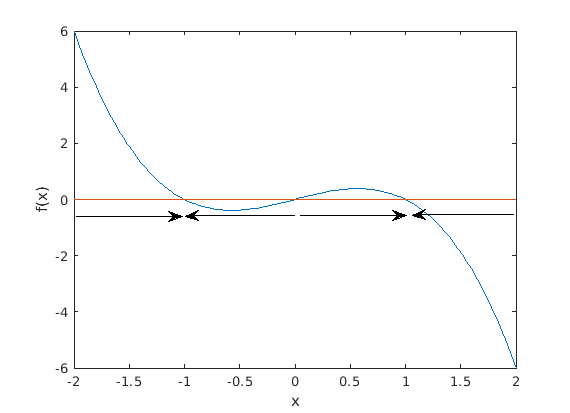
\includegraphics[width=0.6\textwidth]{lista1_7a1.png}
    \caption{Diagrama dos equilíbrios com zonas de atração indicadas por flechas.}
    \label{fig:lista1_7a1-png}
\end{figure}

\begin{figure}[H]
    \centering
    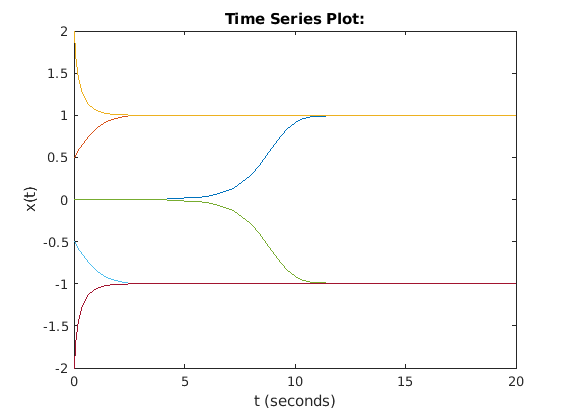
\includegraphics[width=0.6\textwidth]{lista1_7a2.png}
    \caption{Comportamento do sistema para diferentes condições iniciais.}
    \label{fig:lista1_7a2-png}
\end{figure}

Confirmamos a nossa interpretação através da simulação do sistema para diferentes condições iniciais, como visto na figura acima.

\subexercise{c}

\begin{figure}[H]
    \centering
    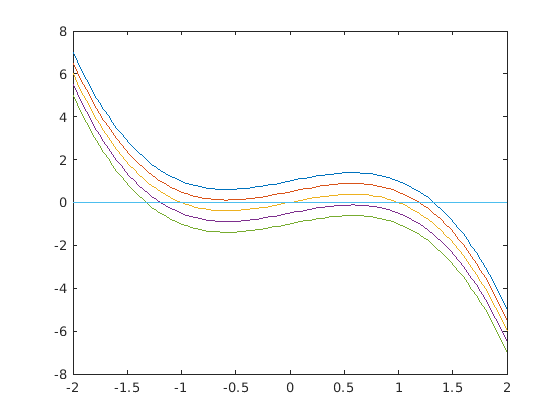
\includegraphics[width=0.6\textwidth]{lista1_7c.png}
    \caption{Comportamento dos equilíbrios e varição do parâmetro $\mu$.}
    \label{fig:lista1_7c-png}
\end{figure}

Vemos que acontece da mesma forma que no exercício 5, entretanto, sempre se mantém pelo menos um equilíbrio estável.

\subexercise{d}

\begin{figure}[H]
    \centering
    \includegraphics[width=0.6\textwidth]{lista1_7d.pdf}
    \caption{Diagrama de bifurcações do sistema.}
    \label{fig:lista1_7d-png}
\end{figure}

\exercise{8}

Podemos definir $x_1 = \theta$ e $x_2 = \dot{\theta}$, o que resulta em um sistema \[
\begin{cases}
    \dot{x_1} = x_2 \\
    \dot{x_2} = \sin x_1\left( a\cos x_1 -1 \right) -bx_2
\end{cases}
.\] 

Claramente vemos que os pontos de equilíbrio são todos em $x_2=0$, entretanto, temos que \[
\dot{x_2} = 0 \implies \sin x_1 \left( a\cos x_1 - 1 \right) = 0
,\] ou seja, temos pontos de equilíbrio triviais em $x_1 \in  \left\{ 0, \pi \right\} $ e também em $x_1 = \cos^{-1} \frac{1}{a}$, que resulta em dois possíveis ângulos no semi-plano superior.

A estabilidade dos equilíbrios pode ser determinada pela Jacobiana do sistema \[
J = \begin{bmatrix} 
    0 & 1 \\
    \cos x_1\left( a\cos x_1 -1 \right) + \sin x_1 \left( -a \sin x_1 \right) & -b
\end{bmatrix} = \begin{bmatrix} 
    0 & 1 \\
    a\cos^2 x_1 -\cos x_1 -a \sin^2 x_1 & -b
\end{bmatrix} 
.\]

Para o ponto de equilíbrio em $x_1=x_2=0$, temos \[
    J = \begin{bmatrix} 0 & 1 \\ 1-a & -b \end{bmatrix} 
,\] que possui autovalores soluções para a equação
\begin{align*}
    \lambda^2 + b\lambda + a-1 = 0 \\
    & \implies \lambda = \frac{-b \pm \sqrt{b^2 -4\left( 1-a \right) } }{2}
,\end{align*}
ou seja, nos permite concluir que o sistema é estável para $a<1$ (dois autovalores negativos).

Para o ponto de equilíbrio em  $x_2=0$ e $x_1=\pi$, \[
    J = \begin{bmatrix} 0 & 1 \\ -1-a & -b \end{bmatrix} 
,\] que possuirá ambos autovalores negativos somente se $a<-1$, uma situação impossível para o sistema real. Entretanto, sabemos que, pela interpretação do sistema, o caso de $a>1$ torna o sistema estável com alguma oscilação, convergindo para  $\theta=\pi$.

Já para os autovalores da forma $x_1=\cos^{-1}\frac{1}{a}$, \[
J = \begin{bmatrix} 
    0 & 1 \\
    -a\left( \sqrt{1-\frac{1}{a^2}}  \right) ^2 & -b
\end{bmatrix}  = \begin{bmatrix} 
    0 & 1 \\
    a - \frac{1}{a} & -b
\end{bmatrix}
,\] portanto, os autovalores determinados pela equação \[
\lambda^2 +b\lambda + \frac{1}{a} -a = 0
\] só são negativos se $a \in (-1,1) \setminus \{0\}$, que, considerando os valores realizáveis, seria $a \in  (0,1)$. Entretanto, os pontos de equilíbrio $x_1=\cos ^{-1} \frac{1}{a}$ só são definidos para $a>1$, ou seja, sempre que eles existem são instáveis.

 \subexercise{b}

\begin{figure}[H]
    \centering
    \includegraphics[width=0.6\textwidth]{lista1_8b.pdf}
    \caption{Diagrama de bifurcação do sistema.}
    \label{fig:lista1_8b-pdf}
\end{figure}

Note que ainda existe o ponto de equilíbrio em $\theta=0$ mesmo em $a>1$, entretanto coincide com o eixo das abscissas.

\subexercise{c}

\begin{figure}[H]
    \centering
    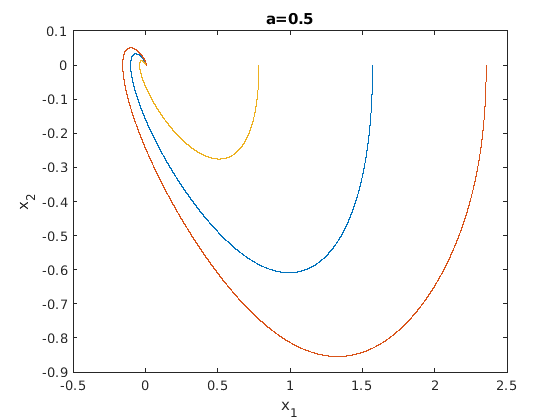
\includegraphics[width=0.6\textwidth]{lista1_8c_1.png}
    \caption{Diagrama de estados para diferentes condições iniciais e $a=0.5$.}
    \label{fig:}
\end{figure}

\begin{figure}[H]
    \centering
    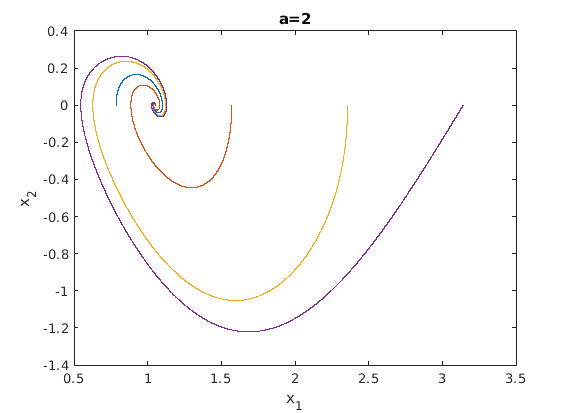
\includegraphics[width=0.6\textwidth]{lista1_8c_2.png}
    \caption{Diagrama de estados para diferentes condições iniciais e $a=2$.}
    \label{fig:lista1_8c_2-png}
\end{figure}

\exercise{9}

\subexercise{a}

Veja que os pontos de equilíbrio do sistema são determinados como \[
    \overline{x} = \frac{-\left( \mu-a \right) \pm \left( \mu-a \right) }{2b}
,\] ou seja, $\overline{x} \in  \left\{ 0, \frac{\mu -a}{b} \right\} $. Agora, a estabilidade dos pontos de equilíbrio pode ser analisada através de
\begin{align*}
    f(x) = \left( \mu-a \right) x -bx^2 \\
    \implies f'(x) = \left( \mu-a \right) -2bx
.\end{align*}
Assim, podemos concluir que o ponto de equilíbrio trivial será estável se $\mu<a$, e para o segundo ponto de equilíbrio \[
    f'(x) = \left( \mu-a \right) -2\left( \mu -a\right) = -\left( \mu-a \right) 
,\] portanto estável somente se $\mu>a$.

\subexercise{b}

\begin{figure}[H]
    \centering
    \includegraphics[width=0.6\textwidth]{lista1_9b.pdf}
    \caption{Diagrama de bifurcações sobre a variação do parâmetro $\mu$.}
    \label{fig:lista1_9b-pdf}
\end{figure}

Os pontos de equilíbrio seguem as equações descritas no item anterior, "invertendo" a estabilidade no ponto $\mu=a$.

\exercise{10}

\subexercise{a}

Em equilíbrio, é evidente que $y=0$, assim, analisando a segunda equação, temos
\begin{align*}
    0 &= \left[ \left( x+1 \right)^2 -\mu  \right] \left[ \left( x-1 \right)^2 +\mu \right] \\
      &= \mu^2 -\left[ \left( x+1 \right)^2 -\left( x-1 \right)^2  \right] \mu -\left( x+1 \right) ^2\left( x-1 \right) ^2
,\end{align*}
ou seja, podemos dizer que existe um ponto de equilíbrio sempre que $\mu =  \left( x+1 \right) ^2$ ou $\mu = -\left( x-1 \right) ^2$. Assim, se $\mu<0$, temos dois equilíbrios em \[
x = 1\pm\sqrt{-\mu} 
,\] enquanto se $\mu > 0$, os equilíbrios serão \[
x = -1 \pm\sqrt{\mu} 
.\] 

Note que, para $\mu=0$, as duas soluções são válidas e os equilíbrios se tornam \[
x = \pm 1
.\] 

\subexercise{b}

\begin{figure}[H]
    \centering
    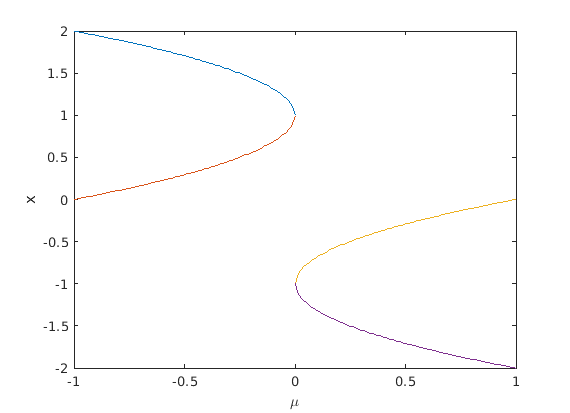
\includegraphics[width=0.6\textwidth]{lista1_10b.png}
    \caption{Diagrama de bifurcações do sistema.}
    \label{fig:lista1_10b-png}
\end{figure}

\exercise{11}

\subexercise{a}

Escolhendo como variáveis de estado \[
\begin{bmatrix} x_1 \\ x_2 \end{bmatrix}  = \begin{bmatrix} y \\ \int \left(  u-y\right)  \end{bmatrix} 
\] podemos escrever o sistema como \[
\begin{cases}
    \dot{x}_1 = -\frac{1}{2} x_1^{s} -\frac{1}{2} x_1+ \frac{1}{2}\sin x_2 \\
    \dot{x}_2 = u-x_1
\end{cases}
,\] em que $x_1^{s}$ representa $x_1$ sob efeito da saturação.

\subexercise{b}

Em equilíbrio, temos 
\begin{align*}
    \dot{x}_2 = 0 \implies x_1=0 \\
    \implies \sin x_2 = 0 \\
    \implies x_2 \in \left\{ 0, \pi \right\} 
.\end{align*}

\subexercise{c}

Primeiro, determinamos a jacobina do sistema, isto é, \[
    J = \begin{bmatrix} -1 & \frac{1}{2}\cos x_2 \\ -1 & 0 \end{bmatrix} 
.\] Para o ponto de equilíbrio $x_2 = 0$, temos  \[
J = \begin{bmatrix} -1 & \frac{1}{2} \\ -1 & 0 \end{bmatrix} 
,\] que possui autovalores determinados pelo polinômio \[
\lambda^2 + \lambda + \frac{1}{2} = 0
,\] ou seja, $\lambda = -\frac{1}{2} \pm \frac{i}{2}$, portanto é um ponto de equilíbrio estável. Já o ponto de equilíbrio $x_2 = \pi$ possui autovalores \[
\lambda = -\frac{1}{2} \pm \frac{\sqrt{3} }{2}
,\] portanto instável.

\subexercise{d}

\begin{figure}[H]
    \centering
    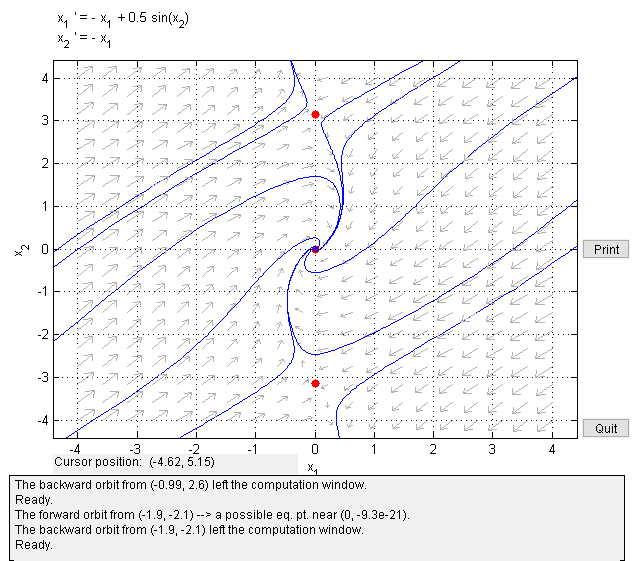
\includegraphics[width=0.6\textwidth]{lista1_11d.png}
    \caption{Diagrama de estados do sistema com pontos de equilíbrio demarcados.}
    \label{fig:lista1_11d-png}
\end{figure}

\exercise{12}

\subexercise{a}

Similar ao exercício 7, os pontos de equilíbrio são $x \in \left\{ 0, 1, 2 \right\} $. A estabilidade do sistema, da mesma forma que nos exercícios anteriores, pode ser determinada a partir do gráfico, que nos indica que somente os pontos de equilíbrio $\left\{ 0,2 \right\} $ são estáveis.

\subexercise{b}

\begin{figure}[H]
    \centering
    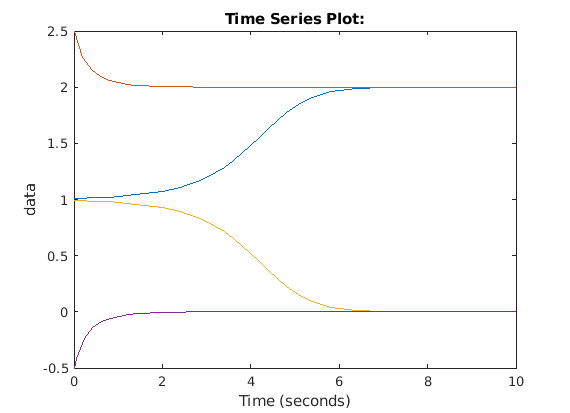
\includegraphics[width=0.6\textwidth]{lista1_12b.png}
    \caption{$y(t)$.}
    \label{fig:lista1_12b-png}
\end{figure}

Conforme indicado já pelo gráfico do enunciado, para qualquer $x(0)>1$, o sistema tenderá a  $x=2$.

\subexercise{c}

\begin{figure}[H]
    \centering
    \includegraphics[width=0.6\textwidth]{lista1_12c.pdf}
    \caption{Diagrama de bifurcação do sistema.}
    \label{fig:lista1_12c-pdf}
\end{figure}

\subexercise{d}


Sabemos que o ponto em que os equilíbrios se tornam imaginários coincide com os mínimos/máximos locais da função $f'$, portanto, \[
    f'(x) = -3x^2 +6x -2 = 0 \implies x = 1 \pm \frac{1}{\sqrt{3} }
.\] Agora, sabemos que o sistema terá somente um ponto de equilíbrio quando, para determinado valor de $u$, $f(1+\frac{1}{\sqrt{3} }, u) <0$, ou seja, $u < -\frac{2\sqrt{3} }{9}$. Da mesma forma, encontramos somente um ponto de equilíbrio quando $u>\frac{2\sqrt{3} }{9}$.

\exercise{13}

Veja que os pontos de equilíbrio do sistema são, além do trivial $r=0$, os pontos em que \[
\lambda + 2r^2 - r^{4} = 0
.\] Ainda mais, podemos realizar a troca de variáveis $x=r^2$ restringindo $x\ge 0$ e entender a equação como um problema de segundo grau, ou seja,
\begin{align*}
    & \lambda +2x - x^2 = 0 \\
    & \implies x = \frac{-2 \pm \sqrt{4 + 4\lambda} }{-2} = 1 \pm \sqrt{1+\lambda}
.\end{align*}

\begin{figure}[H]
    \centering
    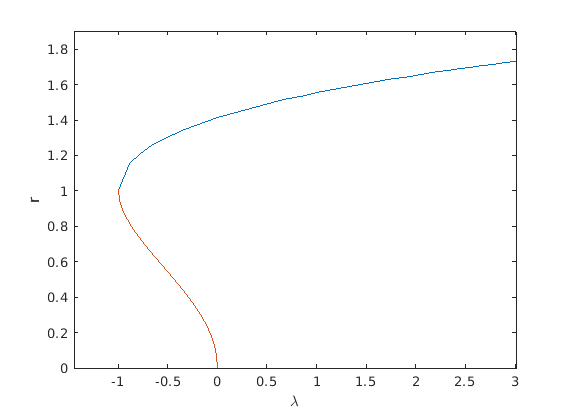
\includegraphics[width=0.6\textwidth]{lista1_13a.png}
    \caption{Diagrama de bifurcação do sistema.}
    \label{fig:lista1_13a-png}
\end{figure}

\subexercise{e}

\begin{figure}[H]
    \centering
    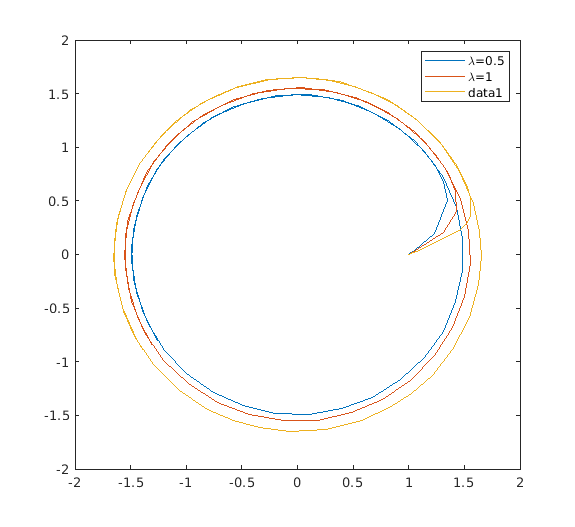
\includegraphics[width=0.6\textwidth]{lista1_13e.png}
    \caption{Diagrama de espaço de estado do sistema após mudança de variáveis para $\lambda \in \left\{ 0.5, 1, 1.5 \right\} $.}
    \label{fig:lista1_13e-png}
\end{figure}

Como esperado, o parâmetro $\lambda$ é correlato ao ponto de equilíbrio estável, influenciando, após a mudança de variáveis, no raio do oscilador.

\exercise{14}

Primeiro podemos aproximar a não linearidade por um ganho  \[
    N(A) = \frac{4}{\pi A}
.\] De forma geométrica, sabemos que o ponto $KG(j)=-2$ representa a interseção entre o diagrama polar do sistema e a função descritiva da saturação, então podemos afirmar que a frequência do ciclo limite, em rad/s é \[
\omega_c = 1
\] pois é a frequência na qual a interseção acontece, e a amplitude do ciclo limite pode ser obtida a partir de \[
-\frac{1}{N(A_c)} = -\frac{\pi A_c}{4} = -2 \implies A_c = \frac{8}{\pi}
.\] 

\begin{figure}[H]
    \centering
    \includegraphics[width=0.6\textwidth]{lista1_14.pdf}
    \caption{Esboço do diagrama de Nyquist.}
    \label{fig:lista1_14-pdf}
\end{figure}
 
\exercise{15}

\subexercise{a}

\begin{figure}[H]
    \centering
    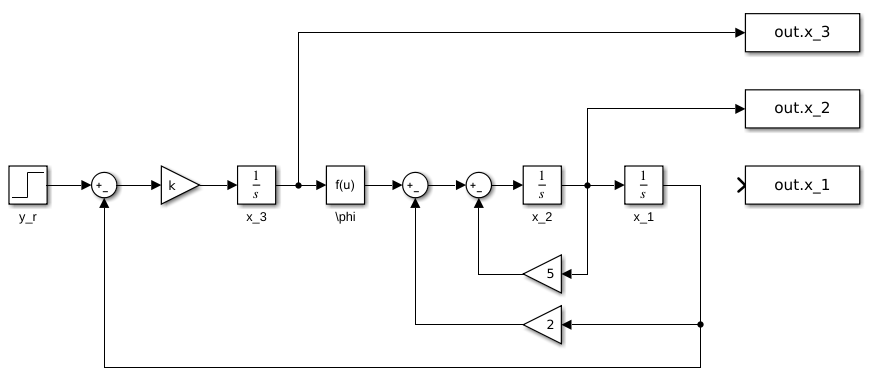
\includegraphics[width=0.6\textwidth]{lista1_15a.png}
    \caption{Diagrama de blocos do sistema.}
    \label{fig:lista1_15a-png}
\end{figure}

\subexercise{b}

Para o sistema se encontrar em equilíbrio, temos
\begin{align*}
    \dot{x}_1 = 0 \implies x_2 = 0 \\
    \dot{x}_3 = 0 \implies x_1 = y_r \\
    \dot{x}_2 = 0 \implies x_3^3 = 6y_r
.\end{align*}

Sua estabilidade pode ser determinada a partir da jacobiana \[
J = \begin{bmatrix} 
    0 & 1 & 0 \\
    -2 & -5 & x_3^2 \\
    -k & 0 & 0
\end{bmatrix} 
,\] cujos autovalores para o ponto de equilíbrio são as raízes da equação \[
\lambda^3 + 5\lambda^2 +2\lambda +kx_3^2 = 0
.\] Utilizando o método de Routh-Hurwitz, montamos a matriz
\begin{center}
\begin{tabular}{c c c}
    1 & 2 \\
    5 & $kx_3^2$ \\
    $10 -kx_3^2$ & \\
    $kx_3^2\left( 10-kx_3^2 \right) $
\end{tabular}
\end{center}
que nos indica que o sistema será estável para
\begin{align*}
    10 - kx_3^2 > 0
,\end{align*}
o que é verdade se $y_r = 0$.

\subexercise{c}

Agora, considerando a variação de $y_r$, temos \[
x_3^2 = \left( 6y_r \right) ^{\frac{2}{3}}
,\] que nos indica que a condição para estabilidade encontrada \[
x_3^2<10
\] se mantém para \[
y_r < \frac{\sqrt{10}^3}{6} \cong 5,27
.\] 

\exercise{16}

Podemos aproximar a função $\phi(x)$ por \[
    \phi(x) = C_0 + \sum_{k=1}^{\infty} A_k\cos k\omega t + B_k \sin k\omega t
.\] Como $\phi$ é uma função ímpar, $A_k = 0 \forall k$, portanto precisamos calcular somente o parâmetro $B$ de sua aproximação. Assim, considerando o ponto de equilíbrio com $y_r = 0$, calculamos
\begin{align*}
    \Phi(t) &\cong B_1\sin\left( \omega t \right) \\
    B_1 &= \frac{1}{\pi}\int_0^{2\pi}\Phi\left( A\sin\tau \right) \sin\left( \tau\right) d\tau ; \tau = \omega t \\
	&= \frac{1}{\pi}\frac{A^3}{3}\int_0^{2\pi}\sin ^{4}\tau d\tau \\
	&= \frac{A^3}{3\pi}\frac{3\pi}{4} = \frac{A^3}{4}
.\end{align*}
Portanto, $\phi$ pode ser aproximado pelo ganho \[
    N(A) = \frac{B_1}{A} = \frac{A^2}{4}
.\] 

Através do diagrama de blocos montado, concluímos que a função de transferência em malha aberta do sistema pode ser representada, sem a não-linearidade, por \[
    G(s) = \frac{k\left( s+5 \right) }{3s\left( s + \frac{10}{3} \right) }
.\] Assim, encontramos os ciclos limites através da equação \[
G(j\omega) = -\frac{1}{N(A)} = \frac{-4}{A^2}
.\] 

\exercise{17}

\begin{figure}[H]
    \centering
    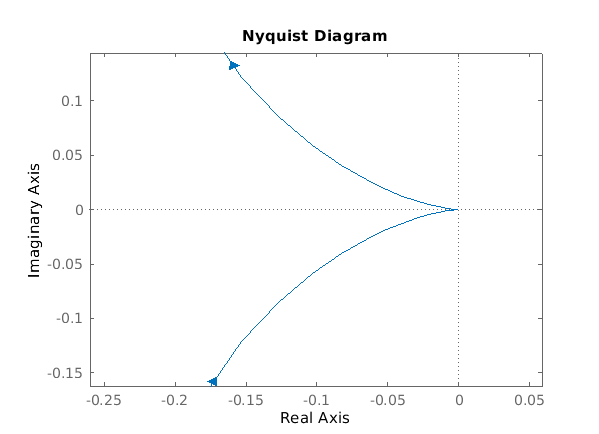
\includegraphics[width=0.8\textwidth]{lista1_17.png}
    \caption{Diagrama de Nyquist de $G(j\omega)$.}
    \label{fig:lista1_17-png}
\end{figure}

Pelo diagrama de Nyquist, podemos observar que não há interseção entre $G(j\omega)$ e a inversa da aproximação da não linearidade, portanto a equação \[
    K*G(j\omega) = \frac{-1}{N(A)}
\] não possui solução, ou seja, não existe ciclo limite.

\exercise{18}

\subexercise{a}

A relação entrada-saída do sistema pode ser descrita como \[
Y(s) = \beta X(s) = \beta \frac{\alpha}{s} U(s)
,\] considerando o atraso, \[
\frac{Y_e(s)}{U(s)} = \frac{\alpha \beta}{s}e^{-sL} = G(s)
.\] O relé pode ser descrito pela função \[
N(A) = \frac{4}{\pi A}
.\] Podemos encontrar um ciclo limite pela equação que aponta a instabilidade do sistema, i.e., \[
1+N(A)G(s) = 0
,\] portanto, \[
G(j\omega) = -\frac{\pi A}{4}
.\] Abordamos essa equação através da magnitude e da fase de ambos os lados da equação
\begin{align*}
    & \varphi \left( -\frac{\pi A}{4} \right) = -\pi \\
    & \varphi \left( G(j\omega) \right) = -\frac{\pi}{2} - \omega L \\
    \implies & \omega_c = \frac{\pi}{2L}
\end{align*}
\begin{align*}
    \|-\frac{\pi A}{4}\| = \frac{\pi A}{4} \\
    \|G(j\omega)\| = \frac{\alpha \beta}{\omega} \\
    \implies A_c = \frac{4 \alpha \beta}{\pi \omega_c} = \frac{8 \alpha \beta L}{\pi^2}
.\end{align*}

\subexercise{b}

\begin{figure}[H]
    \centering
    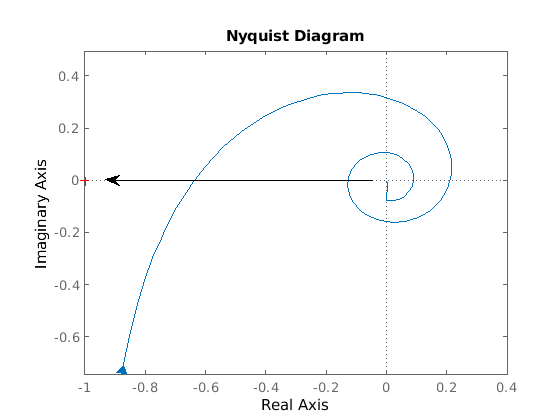
\includegraphics[width=0.6\textwidth]{lista1_18b.png}
    \caption{Diagrama polar do sistema com a inversa da função descritiva representada pela flecha.}
    \label{fig:lista1_18b-png}
\end{figure}

Note que a interseção encontrada é a interseção da esquerda, mais próxima do ponto -1, que é a do ciclo limite. Vemos isso com \[
    A_c = \frac{8}{\pi^2} \cong 0,81 \implies \frac{-1}{N(A)} = -0,64
,\] coincidindo com o gráfico.

\exercise{19}

A existência do ciclo limite é trivial, basta a verificação através da substituição. Para a estabilidade, temos por Lyapunov que a estabilidade é garantida se $V(x)$ é pos-def em relação ao equilíbrio e $\dot{V}$ é (semi-)neg-def. A primeira condição é trivialmente verificada sob as condições $a>0$ e $b>0$. Para a segunda condição, vemos que
\begin{align*}
    \dot{V} &= \nabla V \cdot f(x) \\
	    &= \begin{bmatrix} ax_1 & bx_2 \end{bmatrix} \begin{bmatrix} x_2\left( 1+x_1^3 \right) \\ -3x_1 -3x_1^{4} -x_2^3 \end{bmatrix} \\
	    &= ax_1x_2 + ax_1^{4}x_2 -3bx_1x_2 -3bx_1^{4}x_2 -bx_2^{4} \\
	    &= -bx_2^{4} +\left( a-3b \right) x_1x_2 +\left( a-3b \right) x_1^{4}x_2
.\end{align*}
Assim, vemos que se
\begin{align*}
    b>0 \\
    a=3b \\
\end{align*}
$\dot{V}$ é semi-neg-def, uma vez que $\dot{V}\left( x_1,0 \right) \forall x_1$, portanto, provando que o ponto de equilíbrio é estável.

Agora para analisar a abrangência da estabilidade, vemos que, além do equilíbrio trivial, \[
x_1 = -1 \implies \dot{x}_1 = 0
,\] e também, nesse caso, \[
x_2 = 0 \implies \dot{x}_2 = 0
,\] ou seja, $\left( -1,0 \right) $ também é um ponto de equilíbrio e está dentro das condições de estabilidade do ponto de equilíbrio $\left( 0,0 \right) $, portanto o ponto de equilíbrio é estável somente localmente, sendo o ponto de equilíbrio $\left( -1,0 \right) $ estável ou não.

\exercise{20}

\subexercise{a}

Para o sistema enunciado, claramente o ponto de equilíbrio se dá em $\overline{y}=0$, agora para a segunda equação, temos \[
    \dot{y} = 0 \implies -x^3 -0 = 0 \implies \overline{x} = 0
,\] ou seja, somente o ponto de equilíbrio trivial é possível.

Veja que a jacobiana desse sistema no equilíbrio é \[
    J = \begin{bmatrix} 0 & 1 \\ 0 -4 \end{bmatrix} 
,\] que não nos permite julgar sua estabilidade uma vez que possui um autovalor nulo.

Assim, pela função de Lyapunov fornecida, analisamos que ela é claramente positiva definida para o ponto de equilíbrio. Além disso, podemos ver que
\begin{align*}
    \nabla V &= \begin{bmatrix} x^3 & y \end{bmatrix} \\
    \implies \dot{V} &= x^3y -x^3y -y^2\left( 4-x^2-4y^2 \right) =-y^2\left( 4-x^2-4y^2 \right)
,\end{align*}
ou seja, além de ser nula $\forall \left( x,0 \right) $, ela só é negativa dentro da região demarcada por $\left( x,y \right) : 4-x^2-4y^2 > 0$, i.e., sua região de estabilidade.

\subexercise{b}

\begin{figure}[H]
    \centering
    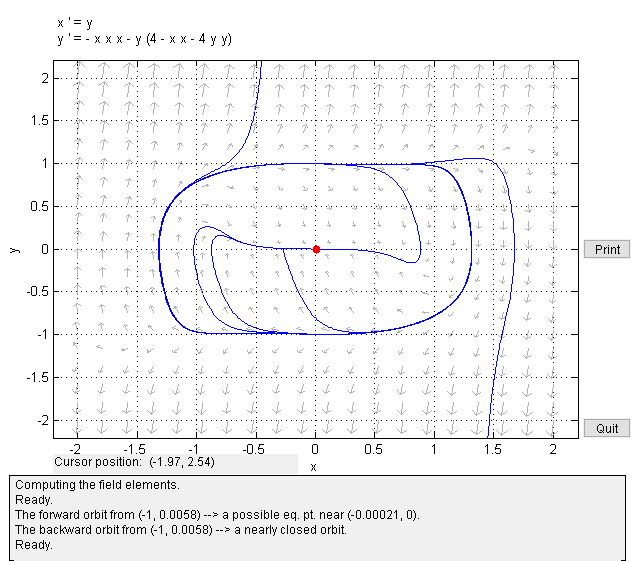
\includegraphics[width=0.6\textwidth]{lista1_20b.png}
    \caption{Região de atração do equilíbrio trivial.}
    \label{fig:lista1_20b-png}
\end{figure}

\exercise{21}

Vide exercício anterior.

\exercise{22}

Sabemos que podemos aproximar o relê por uma função do ganho, i.e., \[
    \phi\left( . \right) \cong N(A) = \frac{4}{\pi A}
.\] Assim, podemos analisar o momento de oscilação, ou seja, no ponto de instabilidade do sistema
\begin{align*}
    1+G(s)\phi(.) = 0 \implies G(s) = -\frac{1}{N(A)}
.\end{align*}
Para uma oscilação, podemos entender $s=j\omega$, o que nos permite chegar à equação
\begin{align*}
    -\frac{\pi A_c}{4} &=\frac{k}{j\omega_c + 1}\exp^{-Lj\omega_c}\\
		       &= \frac{k\left( \cos L\omega_c -j\sin L\omega_c \right) \left( j\omega_c -1 \right) }{-\omega_c^2 -1} \\
		       &= k\frac{\omega_c\sin L\omega_c -\cos L\omega_c}{-\omega_c^2 -1} +jk\frac{\omega_c \cos L\omega_c + \sin L\omega_c}{-\omega_c^2 -1}
,\end{align*}
o que nos permite encontrar o parâmetro $L$ a partir de
\begin{align*}
    &\omega_c \cos L\omega_c + \sin L\omega_c = 0 \\
    &\implies -\omega_c = \tan L\omega_c \\
    &\implies L = \frac{\arctan \omega_c}{\omega_c}
\end{align*}
e o ganho $k$ como
\begin{align*}
    &k\frac{\omega_c\sin L\omega_c -\cos L\omega_c}{-\omega_c^2 -1} = -\frac{\pi A_c}{4} \\
    &\implies k = \frac{\pi A_c \left( \omega_c^2 +1 \right) }{4\left( \omega_c\sin L\omega_c -\cos L\omega_c \right) }
.\end{align*}

\subexercise{b}

\begin{figure}[H]
    \centering
    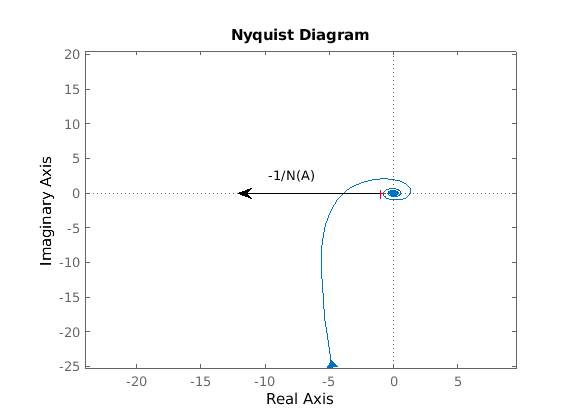
\includegraphics[width=0.6\textwidth]{lista1_22b.png}
    \caption{Exemplo de diagrama polar do sistema, onde a seta representa a inversa da função descritiva do relê e a interseção o ponto de oscilação.}
    \label{fig:lista1_22b-png}
\end{figure}

\subexercise{c}

Aplicando as fórmulas gerais, encontramos \[
\begin{cases}
    L \cong 0,0124 \\
    k \cong 493,5584
\end{cases}
.\]

\exercise{23}

\subexercise{a}

Primeiro, transformamos o sistema para variáveis de estado com $x_1 = \theta$ e $x_2 = \dot{\theta}$ \[
\begin{cases}
    \dot{x}_1 = x_2 \\
    \dot{x}_2 = -x_1 - x_2^3 -\mu x_2 
\end{cases}
.\] Vemos que o sistema possui somente o equilíbrio trivial, para qualquer valor de $\mu$.

Agora, analisamos a jacobiana do sistema  \[
J = \begin{bmatrix} 
    0 & 1 \\
    -1 & -3x_2^2 -\mu
\end{bmatrix} 
,\] que, avaliada no ponto de equilíbrio \[
J = \begin{bmatrix} 
    0 & 1 \\
    -1 & -\mu
\end{bmatrix} 
,\] possuirá autovalores da forma \[
-\frac{\mu}{2} \pm \frac{\sqrt{\mu^2 -4} }{2}
,\] ou seja, ambos estáveis somente para $\mu>0$. Ainda mais, veja que para $|\mu| \le 4$, a parte real dos autovalores coincide.

\subexercise{b}

\subexercise{c}

\begin{figure}[H]
    \centering
    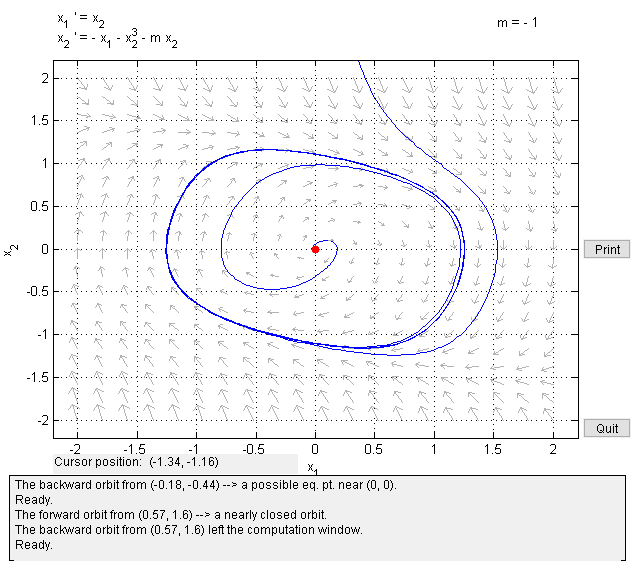
\includegraphics[width=0.6\textwidth]{lista1_23c_l-1.png}
    \caption{$\mu<\mu_c$}
    \label{fig:lista1_23c_l-1-png}
\end{figure}

\begin{figure}[H]
    \centering
    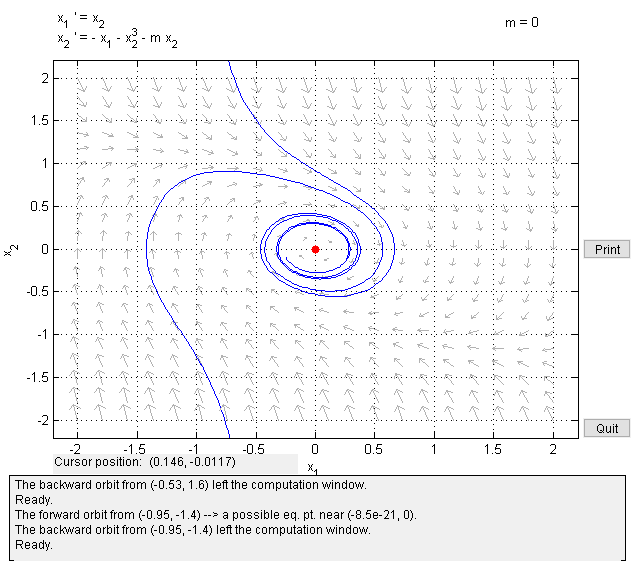
\includegraphics[width=0.6\textwidth]{lista1_23c_l0.png}
    \caption{$\mu=\mu_c$}
    \label{fig:lista1_23c_l-1-png}
\end{figure}

\begin{figure}[H]
    \centering
    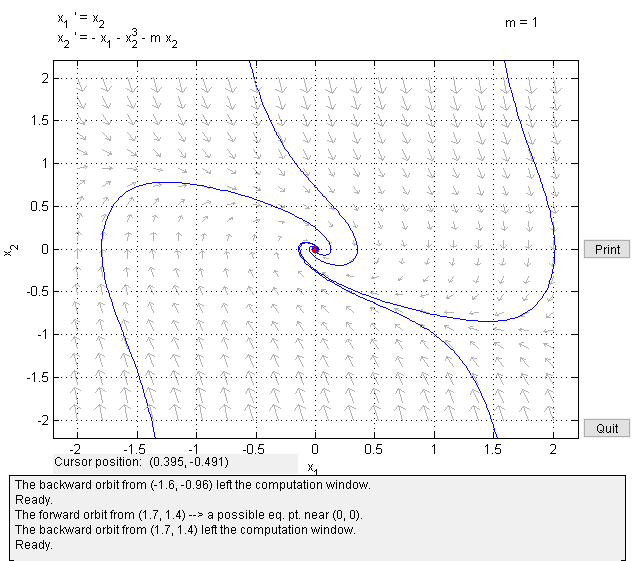
\includegraphics[width=0.6\textwidth]{lista1_23c_l1.png}
    \caption{$\mu>\mu_c$}
    \label{fig:lista1_23c_l-1-png}
\end{figure}

\exercise{24}

\subexercise{a}

Nesse caso, o sistema pode ser modelado como \[
\begin{cases}
    \dot{x} = \frac{1}{L}y -\frac{1}{L}V_a\left( x \right) \\
    \dot{y} = \frac{100}{C} -\frac{1}{C}y -\frac{1}{C}x
\end{cases}
,\] o que nos indica que o equilíbrio é atingido quando
\begin{align*}
    & \dot{x} \implies \overline{y} = V_a(\overline{x}) \\
    & \dot{y} = 0 \implies \overline{y} = V_a(\overline{x}) = 100 - \overline{x}
.\end{align*}
Portanto, podemos obter os possíveis valores de $\overline{x}$ de forma geométrica, pela interseção de $100 - x$ e a curva de $V_a(x)$ fornecida.

Para analisar a estabilidade dos equilíbrios, vemos que a jacobiana é \[
J = \begin{bmatrix} 
    -\frac{1}{L}V_a'(\overline{x}) & \frac{1}{L} \\
    -\frac{1}{C} & -\frac{1}{C}
    \end{bmatrix}
.\] Podemos encontrar os autovalores a partir da equação \[
\lambda = \frac{Tr(A)}{2} \pm \sqrt{\frac{Tr(A)^2}{2^2} -det(A)} 
,\] onde \[
Tr(A) = -\frac{V_a'(\overline{x})}{L} - \frac{1}{C}
\] e \[
det(A) = \frac{V_a'(\overline{x})}{LC} + \frac{1}{LC}
.\] Para garantir estabilidade, precisamos que \[
Tr(A) < 0 \implies V_a'(\overline{x}) > - \frac{L}{C}
\] e 
\begin{align*}
    & \sqrt{\frac{Tr(A)^2}{2^2} -det(A)} < \frac{Tr(A)}{2} \\
    & \implies det(A) > 0 \\
    &\implies V_a'(\overline{x}) > -1
.\end{align*}

Agora veja que o sistema pode possuir até 3 equilíbrios dependendo da interseção entre $100-x$ e $V_a(x)$. A primeira interseção invariavelmente ocorre antes do valor máximo de $V_a(x)$, na parte crescente da curva, o que nos garante que $V_a'(\overline{x}) > 0$ e, portanto, é um ponto de equilíbrio estável. Já os demais equilíbrios acontecem, se existentes, após o pico e, pela característica da curva, podemos afirmar que $V_a'(\overline{x})<0$, ou seja, precisamos de uma análise mais aprofundada para verificar sua estabilidade.

\subexercise{b}

De uma forma mais geral, os equilíbrios são \[
    \overline{y}=0 ; \overline{x} = \frac{1}{R}\left( 100 - V_a(\overline{x}) \right) 
,\] ou seja, $\overline{x}$ pode ser determinado pela interseção das curvas $V_a(x)$ e $100 -Rx$.

\begin{figure}[H]
    \centering
    \includegraphics[width=0.6\textwidth]{lista1_24b.pdf}
    \caption{Esboço dos possíveis equilíbrios do sistema sobre o gráfico de $V_a(x)$.}
    \label{fig:lista1_24b-pdf}
\end{figure}

\subexercise{c}

Vemos que $R\to 0 \implies \overline{x}\to 0$, sendo o único ponto de equilíbrio, e $R\to \infty \implies \overline{x}_1, \overline{x}_2\to x_p : V_a(x_p) = 100$ e $\overline{x}_3 \to \infty$.

\subexercise{d}

\begin{figure}[H]
    \centering
    \includegraphics[width=0.6\textwidth]{lista1_24c.pdf}
    \caption{Esboço do diagrama de bifurcações do sistema.}
    \label{fig:lista1_24c-pdf}
\end{figure}

\exercise{25}

\subexercise{a}

Temos que o equilíbrio do sistema é determinado por \[
0 = \alpha +\mu x - x^3 \implies -\alpha = \mu x - x^3
,\] ou seja, podemos encontrar o equilíbrio pela interseção das curvas $y_1 = \mu x - x^3$ e $y_2=-alpha$.

Agora, para analisar a estabilidade, podemos afirmar que o sistema é estável quando \[
    f'(x) = \mu - 3x^2 < 0 \implies |x| > \sqrt{\frac{\mu}{3}} 
.\] Entretanto, veja que $x = \pm \sqrt{\frac{\mu}{3}} $ são os pontos de inflexão da curva do polinômio de 3º grau, ou seja, seus mínimo e máximo locais. Assim, pela análise geométrica das curvas $y_1$ e $y_2$, podemos afirmar que sempre que o sistema sempre terá pelo menos 1 equilíbrio estável, tendo dois quando $-\alpha$ estiver entre os pontos de inflexão da curva $y_1$.

\subexercise{b}

\exercise{26}

\subexercise{a}

Partindo da análise do diagrama de blocos, tem-se
\begin{align*}
    \psi &= \theta_i - \theta_o \\
	 &= \theta_i - \frac{1}{s}k\sin \psi
,\end{align*}
que, rearranjando os termos, torna-se
\begin{align*}
    -k \sin \psi = s\left( \psi - \theta_i \right) \\
    \implies  \dot{\psi} = f(\psi,\theta_i) = \dot{\theta}_i - k \sin\psi
.\end{align*}

\subexercise{b}

Nesse caso, \[
\dot{\theta}_i = \gamma
,\] portanto, os equilíbrios se dão em \[
0 = \gamma - k \sin\psi \implies \overline{\psi} = \arcsin \frac{\gamma}{k}
.\] Assim, por definição, sabemos que  \[
\|\frac{\gamma}{k}\| \le 1 
,\] o que implica em $\gamma \le k$.

Agora veja que \[
    f'(x) = -k\cos\psi < 0 \forall \psi \in \left( \frac{-\pi}{2}, \frac{\pi}{2} \right) 
.\] Assim, temos que \[
\gamma \in (0,1) \implies \overline{\psi} \in \left( \frac{-\pi}{2}, \frac{\pi}{2} \right) \implies f'(x) \le 0
,\] o que demonstra a estabilidade dos pontos de equilíbrio para $\gamma < k$.

\begin{figure}[H]
    \centering
    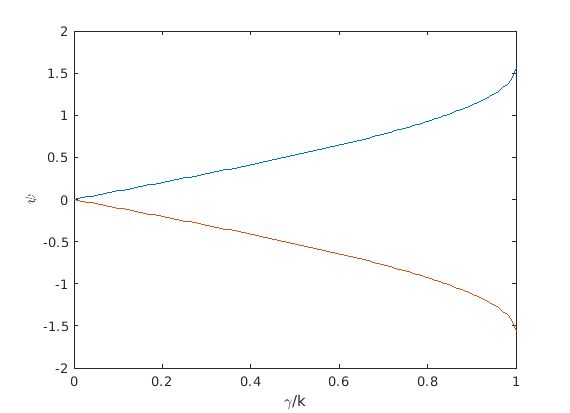
\includegraphics[width=0.6\textwidth]{lista1_26b.png}
    \caption{Diagrama do sistema para entrada de rampa.}
    \label{fig:lista1_26b-png}
\end{figure}

\subexercise{c}

Para um filtro de 2ª ordem, o sistema se torna
\begin{align*}
\psi = \theta_i - \frac{k}{s+a}\frac{1}{s}\sin\psi \\
\implies k \sin\psi = a\left( \dot{\theta_i} - \dot{\psi} \right) + \ddot{\theta_i} - \ddot{\psi} \\
\implies \ddot{\psi} = a\dot{\theta_i} + \ddot{\theta_i}	- a\dot{\psi} -k\sin\psi
.\end{align*}
Usando os estados do enunciado, podemos formular o sistema como \[
\begin{cases}
    \dot{x}_1 = x_2 \\
    \dot{x}_2 = a\dot{\theta_i} + \ddot{\theta_i} - ax_2 -k\sin x_1
\end{cases}
.\] Considerando novamente uma entrada de rampa $\theta_i = \gamma t$, o sistema se torna  \[
\begin{cases}
    \dot{x}_1 = x_2 \\
    \dot{x}_2 = a\gamma - ax_2 -k\sin x_1
\end{cases}
.\] 

Para esse novo sistema, podemos facilmente encontrar o equilíbrio similarmente ao problema anterior como \[
x_2 = 0; x_1 = \psi = \arcsin \frac{a\gamma}{k}
\] e, como podemos realizar a transformação $k' = \frac{k}{a}$ que também $k'>0$, as análises anteriores se mantém.

Para analisar agora a estabilidade do sistema, primeiro ressalta-se que a função candidata deve ser da forma \[
    V(x_1,x_2) = 1 - \cos\left( x_1-\overline{x_1} \right) + \frac{1}{2}Px_2^2
\] para ser positiva definida dentro dos limites de existência do equilíbrio como constatado anteriormente.

Agora, vê-se que 
\begin{align*}
    \dot{V} &= \nabla V f(\bm{x}) = \begin{bmatrix} \sin\left( x_1-\overline{x_1} \right) & Px_2 \end{bmatrix} f(x_1,x_2) \\
    &= \sin\left( x_1 - \overline{x_1} \right) x_2 + a\gamma P x_2 - aPx_2^2 -x_2kP\sin x_1 \\
    &= x_2 \left( a\gamma P - kP \sin x_1 +\sin x_1 \cos \overline{x_1} - \sin \overline{x_1}\cos x_1 \right) 
.\end{align*}

\exercise{27}

Utilizando \[
    V(x,y) = \frac{1}{2}x^2 + \frac{1}{2}y^2
,\] que é claramente pos-def para o ponto de equilíbrio $(0,0)$, temos
\begin{align*}
    \dot{V} &= \nabla V f(x,y) = \begin{bmatrix} x & y \end{bmatrix} f(x,y) \\
    &= -x^2\left( 1-x^2 \right) \left( 1-y^2 \right) -y^2\left( 1-x^2 \right) \left( 1-y^2 \right) \\
    &= -\left( x^2 + y^2 \right) \left( 1-x^2 \right) \left( 1-y^2 \right)
.\end{align*}
Assim, se limitamos $x,y \in \left( -1,1 \right) $, temos que $\dot{V}$ é neg-def para o ponto de equilíbrio proposto. Portanto, localmente assintoticamente estável.

\exercise{28}

\subexercise{a}

Sabemos que o relé pode ser aproximado por  \[
    N(A) = \frac{4}{\pi A}
.\] Ainda mais, podemos encontrar o ponto crítico/de oscilação pela interseção do diagrama de Nyquist do sistema e a reta que representa $N(A)$, analiticamente,
\begin{align*}
    G(j\omega_c) = \frac{-1}{N(A_c)} \\
    \implies \frac{10}{-j\omega_c^3 -2\omega_c + j\omega_c} = \frac{-A_c\pi}{4} \\
,\end{align*}
agora
\begin{align*}
    G\left( j\omega_c \right)  &= \frac{1}{\omega_c}\frac{10}{-2 +j\left( 1-\omega_c^2 \right) } \\
			       &= \frac{1}{\omega_c} \frac{10\left( -2 -j\left( 1-\omega_c^2 \right)  \right) }{4 + \left( 1-\omega_c^2 \right) ^2} \\
			       &= \frac{-20}{\omega_c\left( 4 + \left( 1-\omega_c^2 \right) ^2 \right) } + \frac{-j10\left( 1-\omega_c^2 \right) }{\omega_c\left( 4 + \left( 1-\omega_c^2 \right) ^2 \right)}
.\end{align*}
Igualando os componentes reais e imaginários à outra equação, temos \[
\begin{cases}
    \frac{-20}{\omega_c\left( 4 + \left( 1-\omega_c^2 \right) ^2 \right) } = \frac{-A_c\pi}{4} \\
    \frac{-10\left( 1-\omega_c^2 \right) }{\omega_c\left( 4 + \left( 1-\omega_c^2 \right) ^2 \right)} = 0
\end{cases}
.\] Da segunda igualdade, podemos determinar que
\begin{align*}
    & -10\left( 1-\omega_c^2 \right) = 0 \\
    \implies& \omega_c^2 = \frac{10}{10} \\
    \implies& \omega_c = 1
,\end{align*}
desconsiderando a possibilidade de frequência negativa. Da primeira igualdade, já substituindo o valor de $\omega_c$ encontrado,
\begin{align*}
    & \frac{-20}{4} = \frac{-A_c\pi}{4} \\
    \implies& A_c = \frac{20}{\pi}
.\end{align*}

Assim, projetamos o controlador tendo em vista que \[
T_{osc} = \frac{2\pi}{\omega_c} = 2\pi
\] e \[
K_{osc} = N(A_c) = 0,2
.\] Os parâmetros resultantes são \[
\begin{cases}
    K = 0,12 \\
    T_i = \pi \\
    T_d = \frac{\pi}{4}
\end{cases}
.\] 

\subexercise{b}

\begin{figure}[H]
    \centering
    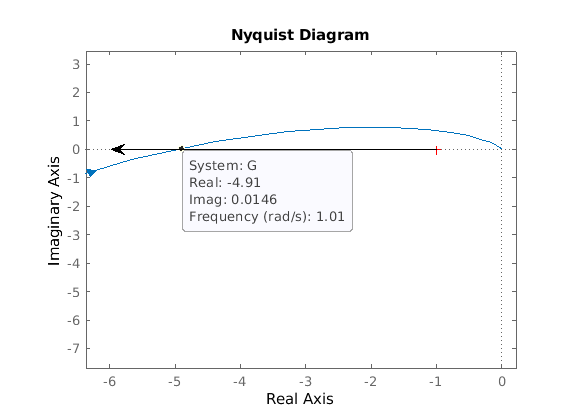
\includegraphics[width=0.6\textwidth]{lista1_28b.png}
    \caption{Diagrama de Nyquist de $G$ em comparação com a inversa da função descritiva $\frac{-1}{N(A)}$, representada pela seta.}
    \label{fig:lista1_28b-png}
\end{figure}

\subexercise{c}

Sem o integrador no sistema,
\begin{align*}
    G\left( j\omega \right) &= \frac{10}{1-\omega^2 +2j\omega} \\
    &= \frac{10\left( 1-\omega^2 -j2\omega \right) }{\left( 1-\omega^2 \right) ^2 +4\omega^2} \\
    &= \frac{10\left( 1-\omega^2 \right) }{\left( 1-\omega^2 \right) ^2 +4\omega^2} + j\frac{-2\omega}{\left( 1-\omega^2 \right) ^2 +4\omega^2}
,\end{align*}
o que resulta nas igualdades \[
\begin{cases}
    \frac{10\left( 1-\omega_c^2 \right) }{\left( 1-\omega_c^2 \right) ^2 +4\omega_c^2} = \frac{-A_c\pi}{4} \\
    \frac{-2\omega_c}{\left( 1-\omega_c^2 \right) ^2 +4\omega_c^2} = 0
\end{cases}
.\] Como a segunda igualdade implica $\omega_c = 0$, não conseguimos utilizar esse método para parametrizar o controlador. A solução mais direta é adicionar um integrador junto do relé.

\exercise{29}

Primeiro, vemos que, de fato, no equilíbrio, \[
\begin{cases}
    \dot{x}_2 = 0 \implies x_1 = -\mu x_2 - x_2^3 \\
    \dot{x_1} = 0 \implies -\mu^2 x_2 -\mu x_2^3 - x_2 -\mu x_2^3 -x_2^4
\end{cases} 
,\] portanto $(0,0)$ é uma solução, logo, um ponto de equilíbrio.

Agora, temos que a jacobiana do sistema \[
J = \begin{bmatrix} 
    \mu +x_2^2 & -1 +2x_1x_2 \\
    1 & \mu +3x_2^2
\end{bmatrix} 
,\] avaliada no ponto de equilíbrio \[
J(0,0) = \begin{bmatrix} \mu & -1 \\ 1 & \mu \end{bmatrix} 
\] possuirá autovalores da forma \[
\lambda = \mu \pm \sqrt{-1} 
,\] portanto temos claramente no ponto $\mu=0$ uma bifurcação de Hopf, onde $\mu<0$ implica em um equilíbrio estável e $\mu>0$ em um equilíbrio instável.

Para viabilizar a análise do sistema, realiza-se a troca de coordenadas retangulares para polares conforme \[
    \begin{cases}
        x_1 = r\cos\theta \\
	x_2 = r\sin\theta
    \end{cases} \\
.\] Assim, as equações do sistema tornam-se 
\begin{align*}
    &\dot{x_1} = \dot{r}\cos\theta -\dot{\theta}r\sin\theta = \mu r\cos\theta - r\sin\theta +r\cos\theta r^2\sin^2\theta \\
    &\dot{x_2} = \dot{r}\sin\theta + \dot{\theta}r\cos\theta = r\cos\theta + \mu r\sin\theta + r^3\sin^3\theta
.\end{align*}
Agora, para encontrar as equações do sistema baseado em $r$ e $\theta$, multiplicou-se ambas por $\cos\theta$
\begin{align}
    & \dot{r}\sin\theta \cos\theta - \dot{\theta}r\sin^2\theta = \mu r\sin\theta\cos\theta -r\sin^2\theta + r^3\cos\theta\sin^3\theta \\
    & \dot{r}\sin\theta\cos\theta + \dot{\theta}r\cos^2\theta = r\cos^2\theta + \mu r\sin\theta \cos\theta + r^3\cos\theta\sin^3\theta
\end{align}
e somou-se de forma que
\begin{align*}
    (1.2) - (1.1) &\implies \dot{\theta}r \left( \sin^2\theta + \cos^2\theta \right) = r\left( \cos^2\theta + \sin^2\theta \right) \\
	      &\implies \dot{\theta} = 1
.\end{align*}
Multiplicando ambas por $\sin\theta$ obtêm-se as equações
\begin{align}
    & \dot{r}\cos^2\theta -\dot{\theta}r \sin\theta\cos\theta = \mu r \cos^2\theta - r\sin\theta\cos\theta + r^3\cos^2\theta\sin^2\theta \\
    & \dot{r}\sin^2\theta + \dot{\theta}r \sin\theta\cos\theta = r\sin\theta\cos\theta + \mu r \sin^2\theta + r^3\sin ^{4}\theta
\end{align}
que podem ser combinadas resultando em
\begin{align*}
    (1.3) + (1.4) &\implies \dot{r}\left( \sin^2\theta + \cos^2\theta \right) = \mu r \left( \sin^2\theta + \cos^2\theta \right) + r^3\left( \cos^2\theta\sin^2\theta + \sin^4\theta \right) \\
	      &\implies \dot{r} = \mu r + r^3\sin^2\theta
.\end{align*}

Dessa forma, chega-se ao sistema \[
\begin{cases}
    \dot{\theta} = 1 \\
    \dot{r} = \mu r + r^3\sin^2\theta
\end{cases}
.\] Vemos, então, que o sistema possui equilíbrios tal que \[
r \left( \mu + r^2\sin^2\theta \right)  = 0
.\] Assim, como $\sin^2\theta > 0$, o equilíbrio só vai existir para $\mu<0$, caracterizando uma bifurcação de Hopf sub-crítica.

\exercise{30}

\subexercise{a}

Veja que \[
\dot{x_1} = 0 \implies x_2 = 0
,\] o que, por sua vez,
\begin{align*}
    & \dot{x}_2 = 0 \implies \sin x_1 + \frac{a}{2}\sin 2x_1 = 0 \\
    \implies & \sin x_1 + a \sin x_1 \cos x_1 = 0 \\
    \implies & \sin x_1 \left( 1 + a \cos x_1 \right) =0
,\end{align*}
ou seja, o equilíbrio se dá nos pontos $\overline{x}_0 = (0,0)$, $\overline{x}_1 = \left(\pi, 0\right)$ ou $\overline{x}_2 = \left( \cos ^{-1}\frac{-1}{a} \right) $.

A estabilidade dos pontos de equilíbrio pode ser determinada a partir da jacobiana \[
J = \begin{bmatrix} 
    0 & 1 \\
    \cos x_1 + a\cos 2x_1 & -b
\end{bmatrix} 
\], que no ponto $\overline{x}_0$ se torna \[
J(\overline{x_0}) = \begin{bmatrix} 0 & 1 \\ 1+a & -b \end{bmatrix} 
,\] ou seja, possui autovalores da forma \[
\lambda = \frac{-b \pm \sqrt{b^2 +4 +4a} }{2}
,\] que só indicaria estabilidade se $a<-1$, o que não é factível. No ponto $\overline{x}_1$,\[
J(\overline{x_1}) = \begin{bmatrix} 0 & 1 \\ a-1 & -b \end{bmatrix} 
,\] uma matriz com autovalores  \[
\lambda = \frac{-b \pm \sqrt{b^2 -4 +4a} }{2}
,\] ou seja, o ponto de equilíbrio $x_1$ é estável somente para $a<1$. Já para os pontos $x_2$, tem-se \[
J(\overline{x_2}) = \begin{bmatrix} 0 & 1 \\ \frac{-1}{a} + a\left( \frac{2}{a^2} -1 \right) & -b  \end{bmatrix} = \begin{bmatrix} 0 & 1 \\ \frac{1}{a} -a & -b \end{bmatrix} 
,\] que possui autovalores da forma \[
\lambda = \frac{-b \pm \sqrt{b^2 -4a +\frac{4}{a}} }{2}
,\] negativos se $a>1$, ou seja, coincide com a condição de existência de $x_2$.

\subexercise{b}

\begin{figure}[H]
    \centering
    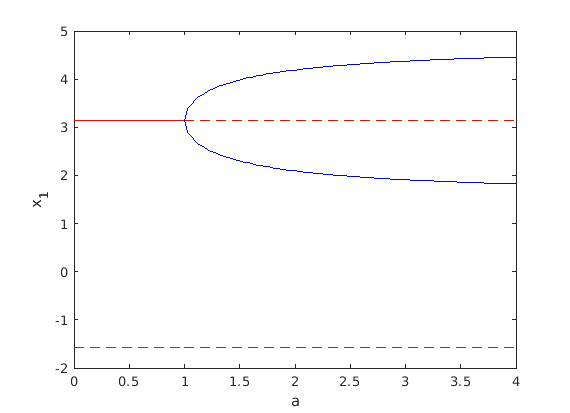
\includegraphics[width=0.6\textwidth]{lista1_30b.png}
    \caption{Diagrama de bifurcações do sistema.}
    \label{fig:lista1_30b-png}
\end{figure}

\subexercise{c}

\begin{figure}[H]
    \centering
    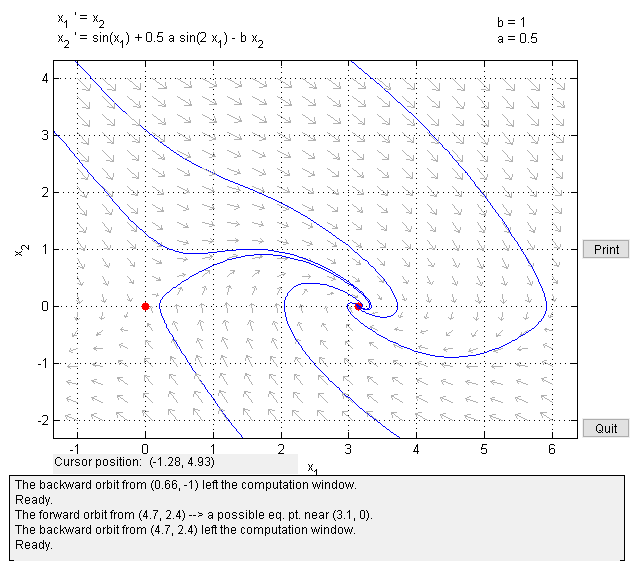
\includegraphics[width=0.6\textwidth]{lista1_30c_0.png}
    \caption{$a=0,5$}
    \label{fig:lista1_30c_0-png}
\end{figure}

\begin{figure}[H]
    \centering
    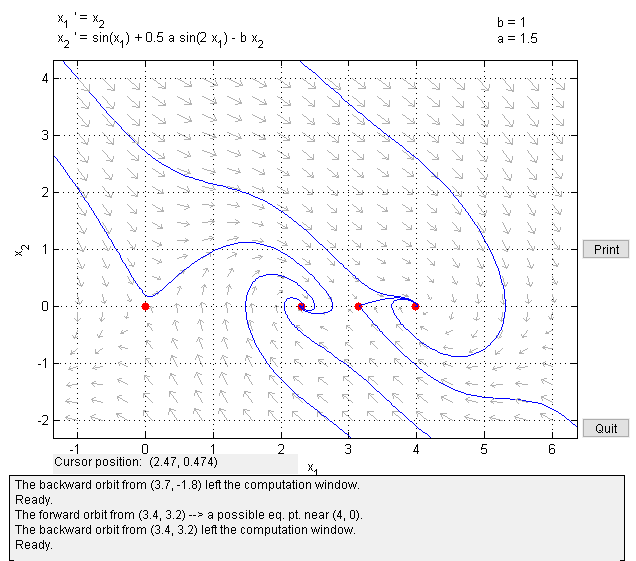
\includegraphics[width=0.6\textwidth]{lista1_30c_1.png}
    \caption{$a=1,5$}
    \label{fig:lista1_30c_0-png}
\end{figure}


\end{document}
